\chapter{Project Discussion}
\label{chp:discussion}
\lhead{Chapter \ref{chp:discussion}. \emph{Project Discussion}}

In this chapter, the project's issues (and their solutions) are discussed in detail, as is the implications and impact of the project as a whole. The various phases of the project provided ample opportunities for problem solving, both in hardware and software as the project's development progressed.

\section{Issues Faced}

During the development of the project, as expected a number of issues were faced and overcome. The probability of unexpected issues arising during the development of any non-trivial project rises exponentially with its complexity, and this project was no exception. The main issues are outlined below, along with the solution chosen.

\subsection{Micropendous Pinout PCB Error}

After the manufacture of the first revision PCB was received some weeks after the order was placed, a problem was discovered in the board layout of the main \textit{Micropendous} microcontroller module. The pinouts of the appeared to have been shifted by one around the entire perimeter of the module. The root issue cause was traced back to the custom Altium component created for the module; for an explicable reason, Altium begins part component schematic pin numbering from pin 0, instead of the conventional pin 1. This resulted in the pin numbering around the module to be rotated by one place.

% TODO: Figures showing incorrect and correct pinouts

Coincidentally, as the unroutable pins were marked as \textit{No-Connect} in the robot schematics (due to their unused functions) the Altium DRC module reported no schematic or routing errors. This resulted in the error not being caught until the board manufacturing had been completed, as a cursory visual inspection of the board layout before production did not catch the subtle pin numbering problem.

While it is possible that the board pinouts could be corrected with manual trace cutting and re-wiring, the scale of the error---some forty pins---and the need for other slight board adjustments forced the decision to produce a second, corrected, version of the PCB.

\subsection{Incorrect Transistor Pinout}

During the component ordering phase of the project, an issue was discovered; no NPN transistors could be found in the appropriate SOT-323 footprint that matched the pinouts given by the Altium library component used. To correct this error, it was necessary to mount the transistors flipped upside-down. This inverted orientation corrected the transistor pinouts (see Figure \ref{fig:flippedtransistor}) so that they could be mounted to the board with the application of a small amount of extra solder to bridge the inverted pins to the PCB.

\begin{figure}[H]
	\centering
		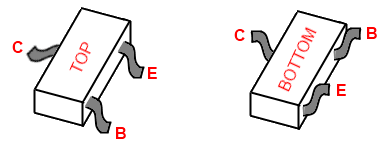
\includegraphics[width=60mm]{FlippedTransistors.png}
	\rule{35em}{0.5pt}
	\caption[Diagram of the normal and flipped SOT-323 Transistor]{Diagram showing the pin-outs of the SOT-323 transistor when mounted normally (\textit{left}) and flipped (\textit{right}).}
	\label{fig:flippedtransistor}
\end{figure}

\subsection{Motor Induced Current Spikes}

During the testing phase of the robot, a failure of the USB AVR microcontroller's USB interface was observed when the motor direction was altered rapidly. Further observation narrowed this down to the switching latency of the chosen inverter transistor (30nS) and H-Bridge (approx. 2$\mu$S). During this time, there exists the possibility of a momentary short in the system battery, if the motor PWM output signal is enabled.

To counteract this, a delay was introduced into the robot's motor driver firmware, to disable the motor output PWM during the switching time. This delay eliminated the high switching current due to the momentary short of the battery, thus preventing the microcontroller USB interface from failing.

Related to the above issue was the motor inrush current, present any time the motor was started from a stationary state. This current, present in all motors under load while the static friction in the motor is overcome, caused large current draw spikes in the main power supply, triggering a destabilization of the main switchmode regulator and thus a brownout of the main microcontroller. This issue was corrected once the main battery was switched from a series of 6 AA cell batteries to a much higher rated Lithium-Ion based battery pack.

\subsection{PCA9306 Physical Package}

Despite having some familiarity with hand-soldering somewhat-small multi-pin surface mount IC components, the package used by the PCA9306 I\superscript{2}C level converter presented a serious challenge. This was due to its US-8 package; measuring just 2.7mm x 4.5mm, the component contains eight pins just .3mm wide each.

Rather than risk destroying the component and waiting additional weeks for a replacement, the LaTrobe University Workshop was requested to use a hot-air gun to solder the device to the robot PCB. This ensured that the component would be correctly placed and soldered without a high risk of component damage. In future projects, relatively cheap components such as this should be ordered with one or more extras added to the quantity, so that damaged components (if any) can be replaced immediately without incurring additional delays while new components are ordered. 

\subsection{L298D Unavailability}

In the first PCB revision, the motor controller design centered around the L298D H-Bridge component, which offered logic level inputs, high current/voltage driver outputs, and convenient internal flyback diodes. These flyback diodes---used to dissipate reverse EMF generated by the motor coils' inductance as they are turned on and off---are a critical part of any such circuit involving inductive loads to prevent damage to the driver.

At the time of ordering however, it was discovered that the L298D variant was not readily available from the University's approved component suppliers. As a second revision of the PCB was already required due to the pinout error of the Micropendous module discussed earlier, a set of external flyback diodes were added on the underside of the board, and the L298N H-Bridge IC used as a substitute. Identical in every other way to the L298D, the L298N variant does not contain internal flyback diodes.

\subsection{Unreliable Bluetooth Packet Buffering}

During development, it was found that occasionally packets sent via the Bluetooth interface were (apparently) being ignored by the receiving device --- this was especially apparent during the L2CAP layer channel initialization and configuration phases. In many instances, a channel would fail to configure at all, causing the remote device connection to time out.

After further investigation, it was determined that the problem source was the lack of a reliable packet buffer within the device; if a packet was delayed within the external Bluetooth HCI controller silicon, the controller would reject new packets for transmission. Without a buffer, these rejected packets for transmission would be lost. Ideally, this could be solved by indicating to the controller that only buffer-related event packets should be returned to the host while the controller is busy, to allow for a polled busy-wait scheme to be used to determine the controller's readiness. However, there is no mechanism to delay incoming L2CAP data packets from the controller during this stage in the HCI specifications, which could potentially result in dropped received packets.

To solve this, the stack's L2CAP layer was extended to include its own internal reliable packet transmission scheme, in the form of a small event queue. As channel events were received or generated internally, the pending event would be added to a reliable queue. When a transmission is attempted, these events are only removed from the queue if the transmission was successful (see Chapter \ref{chp:btstackimp}).

This scheme results in a reliable L2CAP layer, without the use of a large internal packet buffer within the device. Additional similar schemes could potentially be added to the higher level service layers, however this was not found to be necessary for the project's firmware.

\subsection{PS3 Controller Compatibility}

Sony's \textit{Playstation 3} controller presented several small difficulties in making it compatible with the rest of the system. While the controller itself implements the standard HID profiles in both wired USB and wireless Bluetooth modes, additional device-specific software tweaks are necessary for compability.

When plugged in as a wired controller via the USB interface, a special HID Feature packet must be sent to the controller over the logical HID interface, via the USB Control endpoint. This packet, directed to the HID report ID \texttt{0xF4} and containing the special ``magic'' bytes \texttt{0x42 0x0C 0x00 0x00}, it is used to enable general controller reports through the regular HID data endpoints. Without this packet, the controller will not send any state change information to the host. In Bluetooth mode, the magic packet required for Bluetooth HID reporting is \texttt{0x42 0x03 0x00 0x00}.

A second packet during initialization is also required, another HID Feature packet directed at the HID Report ID \texttt{0xF5}. Prefixed with the bytes \texttt{0x01 0x00}, this request packet data is followed by the six octets of the host's Bluetooth device address, to pair the controller to the specified address. This is in contrast with the general Bluetooth pairing mechanism, which usually involves a device discovery and authentication phase over the Bluetooth link.

The two initialization packets for USB HID reporting and Bluetooth address pairing are shown in Listing \ref{lst:ps3hidinit}.

\lstinputlisting[float=tbph,caption={Playstation 3 specific initialization code.},label={lst:ps3hidinit}]{./Figures/PS3SpecificInit.c}

\section{Project Significance}

This project represents a significant impact to the open source and embedded systems communities. It gives a free, open source Bluetooth stack in a new form, paving the way for a new generation of low cost Bluetooth devices. These new devices, using low powered processors previously deemed unsuitable for the task of complex Bluetooth interactions, will give users a new rich landscape of system integration and communication.

While other wireless technologies already in use will remain just as important as they are today, this project gives a new avenue of development for products that can interact directly with off-the-shelf consumer devices. Modern smart-phones, tablet computers and laptops now contain Bluetooth radios as standard features; the stack presented in this project will open up these devices to direct communication with embedded systems without the need for obscure wireless transceiver dongles. In the future, this type of technology will allow for system monitoring and configuration over a wireless link with compatible consumer devices using a rich UI, instead of wired solutions or expensive local displays and buttons.